%\documentclass[12pt]{article}
\documentclass[conference]{IEEEtran}
%\usepackage[title]{appendix}
%\usepackage[T1]{fontenc}
%\usepackage[latin9]{inputenc}
\usepackage{geometry}
\geometry{verbose,tmargin=1cm,bmargin=2cm,lmargin=1cm,rmargin=1cm}
\bibliographystyle{IEEEtran}

%\setlength{\parindent}2}
\usepackage{amsmath}
\usepackage{amssymb}
\usepackage{caption}
\usepackage{adjustbox}
\usepackage{graphicx}% http://ctan.org/pkg/graphicx
\PassOptionsToPackage{normalem}{ulem}
\usepackage{ulem}
\usepackage{setspace}
%\linespread{1.5}
\usepackage{algorithm}
\usepackage{enumitem}
\setlist[enumerate]{label*=\arabic*.}
\usepackage{algpseudocode}
\usepackage{hyperref}
\usepackage{listings}
\usepackage{amsmath}
\usepackage{graphicx}
\hypersetup{
	colorlinks = True,
	linkcolor = blue,
	anchorcolor = blue,
	citecolor = blue,
	filecolor = blue,
	urlcolor = blue
}
\usepackage{amsthm}
\usepackage{setspace}

% \usepackage{titlesec}
% \titleformat{\section}
%   {\normalfont\normalsize\bfseries}{\thesection.}{1em}{}
% \titleformat{\subsection}
%   {\normalfont\normalsize\itshape}{\thesubsection.}{1em}{}
% \titleformat{\subsubsection}
%   {\normalfont\normalsize\itshape}{\thesubsubsection.}{1em}{}

\newtheorem{definition}{Definition}
\newcommand{\R}{\mathbb{R}}
\renewcommand\thesubsection{\Alph{subsection}}
\makeatletter
\date{}

\makeatother

\usepackage{babel}
\begin{document}

\title{Unsupervised Electroluminescence Image Clustering for Automated Defect Detection in Photovoltaic Cells}
  %  \date{\today} 
	
 %\author{\href{mailto:bgp12@case.edu}{Benjamin G. Pierce}$^{1, \dagger}$,
 %       \href{mailto:rxc542@case.edu}{Rounak Chawla}$^2$, and 
 %       \href{mailto:enw30@case.edu}{Ellis Wright}$^2$\\\\
 %       Case Western Reserve University\\
 %       $^1$ Department of Materials Science and Engineering\\
 %       $^2$ Department of Computer and Data Sciences\\\\
        

 %       Sandia National Laboratories\\
 %       $^\dagger$ Photovoltaic Systems Evaluation Laboratory 
        
        %$^3$ Department of Electrical and Computer Engineering
%        }

 \author{\IEEEauthorblockN{Benjamin G. Pierce$^{1, 2}$, Rounak Chawla$^1$, and Ellis Wright$^1$}
 	\IEEEauthorblockA{$^1$Case Western Reserve University, Cleveland, OH, 44106}
    \IEEEauthorblockA{$^2$Sandia National Laboratories, Albuquerque, NM, 87185}
 	}

\maketitle
\begin{abstract}

Photovoltaics (PV) have become an increasingly inexpensive source of renewable energy in recent years, largely due to maturing technology and economies of scale. 
As the total amount of solar PV installed exceeds 1 terawatt (as of 2022), quantification of PV performance becomes crucial to manufacturers, insurers, and system operators. 
A commonly used form of nondestructive testing of PVs is electroluminescence (EL) imaging, where a bias is applied to a PV cell or module and the usable area emits light in the near-infrared spectrum, which is captured by a sensitive camera. 
These EL images are commonly used to manually and qualitatively evaluate modules by the failures or flaws they exhibit, commonly cracking, corrosion, or various manufacturing defects. 
However, it is difficult to do this at scale, especially in an assembly line fashion. 
Previous works have explored the possibilities of using convolutional neural networks (CNNs) to automatically classify EL images, but these CNNs require labeled training data in large quantities, and are vulnerable to the imbalanced class problem. 
In this work, we introduce a unsupervised convolutional auto-encoder (CAE) model, and compare it to a classical unsupervised image processing approach. 
We show that unsupervised approaches can attain very good accuracy scores on an EL image dataset without the need for costly training data with labels.
\end{abstract}

\begin{IEEEkeywords}
electroluminescence imaging, defect detection, photovoltaic characterization, image processing, convolutional autoencoder
\end{IEEEkeywords}

\section{Introduction}
As the world moves towards renewable and reduced emissions energy sources, photovoltaics (PV) have become a economically dominant technology, as the price on PV modules continues to fall. 
The variable cost of fuel (sunlight) for PV is zero, but the large upfront capital expenditure of PV makes it an amortized asset, meaning that in order to be financially viable, a PV system must have a long expected lifetime. 
Defects in PV modules, introduced in manufacturing, shipping, or in the field, can significantly reduce system lifetime. 
Therefore, there is a enormous economic interest in detecting and measuring possible defects in a PV module before, during, and after its lifetime in the field. 


One measurement that is used for this purpose is electroluminescence (EL), which generates an image of the PV module that quantifies how well it can produce electricity. 
The physics behind an EL image is relatively straightforward. 
When operating, a solar panel generates electricity through the photovoltaic effect, where light provides the necessary energy for electrons in the valence band of the module material (boron or phosphorus doped silicon) to excite beyond their valence band and become free electrons, which can move across a p-n junction to induce a current. 

If this is run in reverse and a current is \textit{applied} to the PV panel, it will then \textit{emit} light in the near-infrared spectrum, but only in areas where it would have produced light in normal operation. 
This makes an EL image a valuable measurement of the module, as dark areas in the image correspond to where the module does not produce power. 
This procedure is commonly used as part of an assembly line quality assurance step, or as a field measurement to evaluate module lifetime. 
In either case, evaluation of when a EL image looks different from the ordinary is a useful step to automate, and if needed, evaluate manually. 


However, manual inspection of many EL images is quite costly, and as the PV industry continues to scale up in near short term, the industry needs methods to perform automated review of EL images. 
The literature over the last few years has been focused on using Convolutional Neural Networks (CNNs) to classify EL images based on labeled examples, as in \cite{akram_cnn_2019}. 
This methodology essentially automates the processing of selecting filters in the spacial domain by learning convolutional kernels from the data. 
However, CNNs are very dependent on data quantity and quality, and in particular are vulnerable to the imbalanced class problem, where a dataset does not contain an adequate balance of the intended targets. 
This results in a model learning a non-useful target distribution.
For example, a model trained on a dataset with 999 EL images that represent a "Good" module, and 1 that represents a "Bad" module, the model will be correct 99.9\% of the time by simply always classifying any input as "Good".
While representative of the training set, this output is not desirable. 
Unfortunately, this scenario is very common in EL image data, as manufacturing and operations and maintenance procedures are designed for a low failure rate in order to be profitable, and companies are generally reluctant to perform destructive testing on a large scale, which would be needed to construct a complete, class-balanced dataset for supervised learning. 
Additionally, failures in PV modules can be quite diverse, and difficult to classify into well-defined classes due to different module types, manufacturing processes, and varied failure triggers in the field. 
Even expert labeling of EL images is often subjective and subject to various errors. 
These issues make supervised models like CNNs less desirable for some applications. 

Consider Deitsch \textit{et. al.} \cite{deitsch_automatic_2019}, who developed an EL image dataset of 2624 solar cells, with annotated defect regions. 
This dataset was generated via manual annotation of the ground truth defects in the EL images with the help of an expert. 
While this led to the creation of a useful open dataset, this procedure is inefficient, non-reproducible, and inaccessible to researchers without an expert. 
As such, many unannotated EL image datasets of solar cells exist, and our project aims to examine the the representative accuracy of learned defect features from these datasets in an unsupervised setting.


Unsupervised learning, in contrast, does not require labeled training data, and seeks to estimate the natural clusters in the data, which hopefully correspond to real-world classifications. 
As they are primarily data-driven, unsupervised models can avoid human bias in the labels, and identify failure types that may not be understood \textit{a priori}. 
Additionally, clustering methods can be more robust to imbalanced classes, and are often more explainable when a misclassification occurs. 
However, the main strength of unsupervised methods in this case is in exploratory data analysis and human-in-the-loop feedback. 
Oftentimes, if a model can be used to raise a flag that a certain module has some defect, it is usually inspected manually. 
The value of automated efforts such as this is to narrow the amount of samples that require human intervention, not to replace the human element entirely, while avoiding injection of bias in a labeling process and the associated increased costs of labeling. 
Therefore, in this work, we present two types of unsupervised feature extractors, one that uses classical image processing techniques and one with a deep autoencoder model. 
By comparing these techniques to each other, we can identify which techniques perform the best across various datasets and provide actionable insight and model guidelines/code for use in industry. 
In summary, this work presents the following notable contributions:
\begin{enumerate}
    \item A classical feature extraction pipeline that does not ultilize machine learning
    \item A Convolutional Autoencoder feature extraction pipeline using state-of-the-art ML techniques
    \item Feature vector clustering methods and comparison between various approaches
    \item Performance quantification of methods
\end{enumerate}

\section{Dataset}
There are multiple open EL image datasets available. 
The first is from CWRU, and hosted on OSF \cite{noauthor_osf_nodate}. 
Another dataset \cite{chen_automated_2022} from Lawrence Berkeley National Lab is hosted as part of the Duramat Consortium (which BGP is affiliated with), primarily focusing on crack detection. 
Deitsch \textit{et. al.}'s open EL dataset \cite{deitsch_automatic_2019} predates the former datasets, and is another benchmark in the community. 

\section{Methodology}
The overarching method has the following steps:
\begin{enumerate}
    \item Compute a feature vector $v \in \R^k$ from an image $I \in \R^{m \times n}$, where $k$ is a hyper-parameter that is empirically determined. 
    \item Assemble feature vectors for all $N$ images, forming a matrix $X \in \R^{N \times k}$.
    \item Cluster on the samples, and group each image into a cluster $1...g$, where $g$ is the desired number of groups.
    \item Map each $g_i$ to a corresponding real-world, physical classification.
\end{enumerate}
Step 1 will be performed with A) Classical Image Processing, and B) Deep Learning, which are explained below.
\subsection{Classical Image Processing}
The classical image pipeline will follow that of our previous work in \cite{pierce_identifying_2020} where an image processing \& feature extraction pipeline is constructed to perform clustering on representative vectors of EL images. 
These vectors are extracted with a customized feature detector, which will be improved upon in this paper.
A block diagram of the pipeline is shown in Figure \ref{fig:pipeline}.
\begin{figure}[h]
    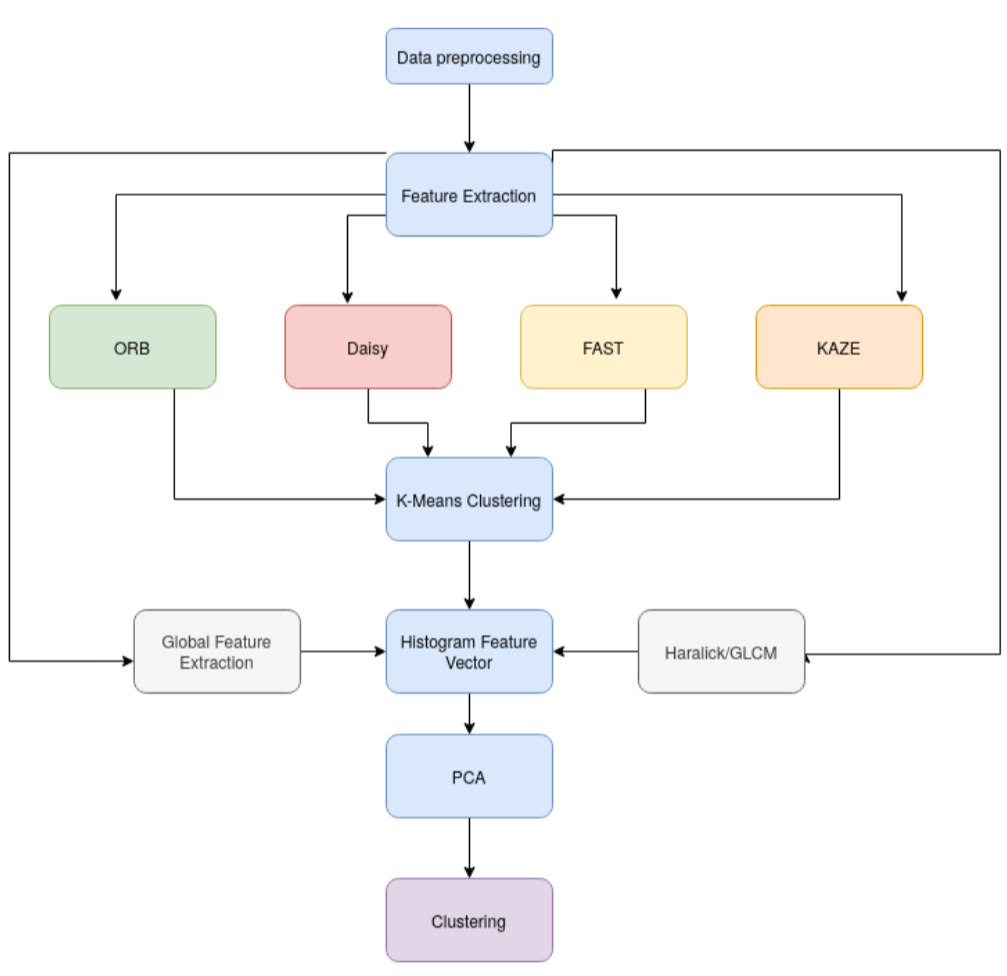
\includegraphics[width=10cm]{pipeline.png}
    \centering
    \caption{The unsupervised classical image processing framework shown in \cite{pierce_identifying_2020}.}
\label{fig:pipeline}
\end{figure}

The first step of the classical image processing pipeline is feature extraction, consisting of three different methods. 
One method is that of local feature extraction, where ``patches" of the image are identified and vectorized by intensity. 
Note that this process is very local, and only operates on patches in order to retain scale and rotation invariance. 
Methods like ORB \cite{rublee_orb_2011}, Daisy \cite{tola_daisy_2010}, FAST \cite{rosten_faster_2010}, and KAZE \cite{alcantarilla_kaze_2012} can all be used interchangeably. 
These methods present generalized approaches; two further methods are used as more application-specific additions to these patch feature extractors. 

Another set of features are known as Haralick or Grey Level Co-occurance Matrix (GLCM) texture features \cite{haralick_textural_1973}. 
These features are more specific to this problem space, as they are restricted to greyscale images. 
Haralick features work by computing dissimilarity and correlation between images patches. 
This process is more direct and a better judge of image texture then the generalized patch feature extractors. 

The final set of features utilized is very specific to this problem. 
Note that the previous two methods operated only on image patches; this can be an issue for this domain, since many features of interest (cracks, corrosion) in EL images stretch over much of the image. 
The final method of ``global feature extraction" is quite simple: take a column-wise sum over the entire image, and normalize this vector between zero and one. 
This concept was first presented in \cite{karimi_generalized_2020} as ``normalized busbar width", where it was noted to correlate with a drop in power due to corrosion. 
This work adapts the process to form a feature vector that can easily delineate the corrosion failure mode. 
\begin{figure}[h]
    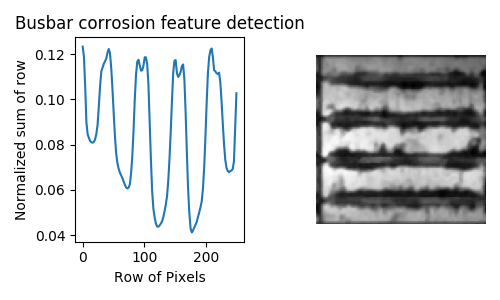
\includegraphics[width=9.5cm]{global_feats.png}
    \centering
    \caption{A vector captured by a column-wise sum over the image and then normalized. This roughly corresponds to the width of the busbars.}
\label{fig:pipeline}
\end{figure}

Once the three feature vectors (one from the patch feature extractor, one from Haralick/GLCM features, and one from the busbar corrosion global detector), they are directly appended together to form a very long vector for each image. 
This vector is generally quite unwieldy and high-dimensional; Principal Component Analysis (PCA) is then employed to shorten it. 
Since the three methods all attempt to quantify the same thing, there is signifigant co-linearity within the merged feature vector. 
This allows PCA to reduce the dimensionality by roughly an order of magnitude, although the exact length of the feature vector is dependent on the data and empirical judgement. 
The reduced feature vector is then used as input the the clustering  metric. 

\subsection{Deep Learning}
In this work, we will use a Convolutional Autoencoder (CAE) as the deep learning technique. 
A CAE learns many convolution kernels to automate the process of feature extraction by down-sampling a image to a vector, thereby creating a representational "bottleneck", and then up-sampling the image back up with transposed convolutions. 
The loss between the original image and reconstructed image is computed, and then backpropagated through the network to learn convolutional kernels. 
These convolutional kernel parameters can be similar to kernels constructed by a classical image processing methodology, but often become difficult to interpret in deeper networks. 

Once the model has been trained to the point where it can successfully reproduce an image, the vector "bottleneck," referred to as the latent space, is used as a vector representation of the image. 
This process can be viewed as a non-linear and high-dimensional version of Principal Component Analysis (PCA), which is commonly applied on vector data for dimensionality reduction by exploiting co-linearites in the data \cite{kramer_nonlinear_1991}. 
Note that the size of the latent space is a significant hyper-parameter for CAE/VAE models, and is a somewhat arbitrary and empirical choice to be optimized with a hyper-parameter tuning framework. 

The architecture of our model is loosely based on the U-Net design from \cite{DBLP:journals/corr/RonnebergerFB15}, and also draws concepts from the Variational Autoencoder from \cite{Subramanian2020}, both of which feature many convolutional layers with a latent space representation of the model. 
Typically, this latent space is a relatively small vector; by forcing information to flow through the latent space to reconstruct the original image, the model learns a low-dimensional encoding of the image data, which is what we were looking for. 
Note that reconstructive step is less important for this application, and is only used as a model training tactic. 

We choose to employ the variational trick such that the decoding half of the network also learns a denoising process, making our model into a ``Variational Autoencoder" (VAE). 
This enables to model to function in a \textit{generative} fashion; if we provide the model with noise at the latent space, it will decode that noise into a plausible image. 
This work does not make use of this feature, but the variational method is still employed because it has been empirically found to be more stable in an EL image context. 
A possible explanation for this is that the optimization of a VAE relies on the evidence lower bound (ELBO) optimization strategy for the log-likelihood of the data. 
The mechanics of this strategy result in the model slightly overfitting the data, which may be desirable behaviour in this case \cite{shekhovtsov2022vae}. 
The output of the model also features the characteristic blurring of the VAE as seen in Figure \ref{fig:recon}; this property does not make a difference in this application as we do not utilize the reconstruction process for generation. 
For realistic generation, adversarial methods \cite{plumerault_avae_2020} may be employed at the cost of training stability; we declined to use them in this work due to the small dataset size. 
Our full architecture is shown in detail in Figure \ref{fig:CAE}; although following a somewhat standard structure, the model is original to this work and therefore does not utilize pre-trained weights or other forms of transfer learning. 

\begin{figure}[h]
    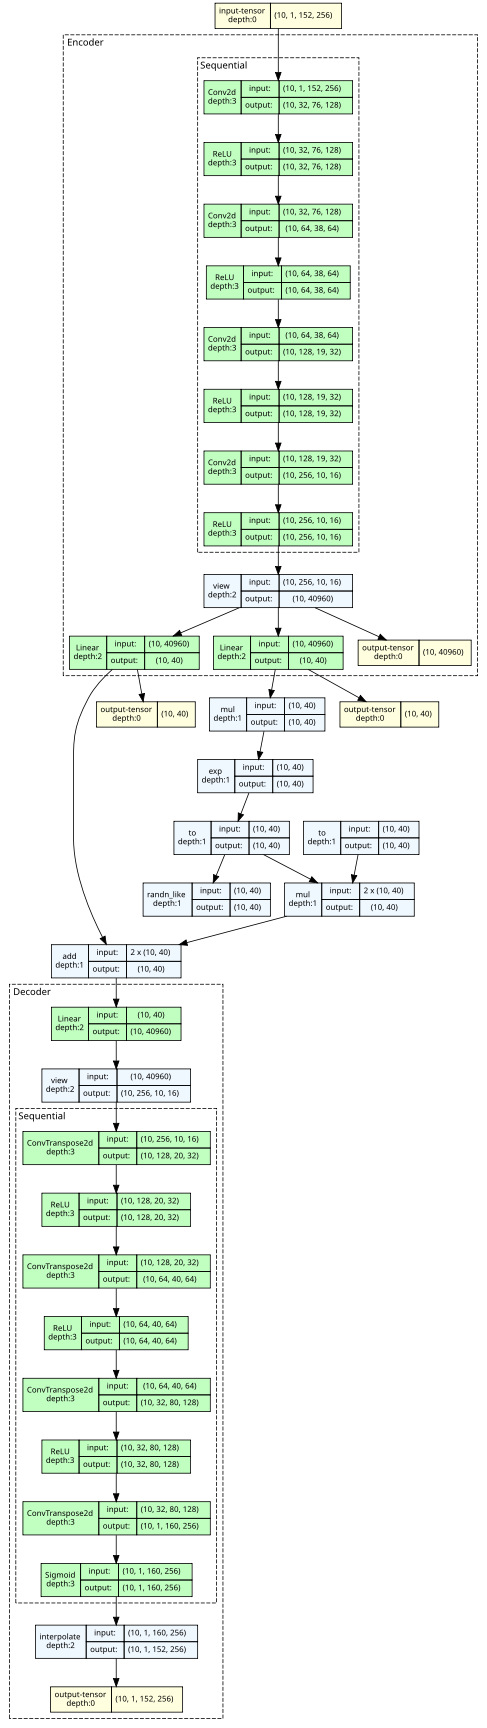
\includegraphics[width=5cm]{modelpic.png}
    \centering
    \caption{The full model architecture of our Convolutional Autoencoder, with image shapes shown for a arbitrary input.}
\label{fig:CAE}
\end{figure}

In any case, the resultant output of the model is a feature vector extracted from the encoder half of the autoencoder of the desired length. 
Therefore, both the classical image processing and machine learning pipelines output a matrix of feature vectors, where each vector corresponds to a single image. 
This matrix is then passed to a clustering method. 

\subsection{Clustering}
%For both feature extraction models, we will cluster the output feature vectors using Gaussian Mixture Models (GMMs), a probabilistic clustering algorithm.
%Other clustering methods, such as $k$-means, $k$-medioids, hierarchical, or density-based may also be explored, depending on model performance. 
%As most are implemented using the scikit-learn Python package, they are somewhat interoperable and swappable. 
In this work, we deploy various clustering algorithms. 
The first the Gaussian Mixture model. 
This algorithm assumes that the data is drawn for a mixture of Gaussian distributions, and seeks to estimate the probability that each point belongs to a certain cluster via expectation maximization \cite{dempster_maximum_1977}. 
This approach provides a more flexible approach then simpler methods like $k$-means\footnote{$k$-means is in fact a special case of GMMs where variance is assumed to be spherical}, but does assume that the data comprises of a mixture of Gaussians. 
This may not always be the case, especially in a high dimensional space.

Another clustering method of interest is hierarchical clustering, which is also known as ``agglomerative" or ``divisive" clustering, depending the implemented approach \cite{szekely_hierarchical_2005}. 
The agglomerative approach begins by assigning samples to their own cluster, and then merges clusters based on a distance metric. 
In contrast, the divisive approach places all samples in one cluster, and then splits that cluster based on a distance metric. 
Both cases utilize some form of distance metric, which can be any valid metric over a defined metric space. 
This is an advantage of hierarchical clustering; in higher dimensional spaces, Euclidean distance is quite poor and it is usually better to use something like $L_1$ (Manhattan/taxicab) distance \cite{domingos_few_2012}, which we utilize in this work. 


\subsection{Comparative Analysis}
In this step, the different models are compared with each other. 
It is expected that each model will have multiple variations that have small, but significant differences, such as different deep learning hyperparameters, different clustering methods, and different filter coefficients. 

Note that comparing unsupervised learning methods is quite difficult, in that human labeled samples may not exactly map to clusters a unsupervised algorithm determines. 
However, this does not strictly imply that the algorithm itself is incorrect; it is quite common for unsupervised methods to pick up on intra-dataset variance that was not identified in \textit{a priori} labeling. 
This represents both an advantage and disadvantage of unsupervised ML. 
For example, in an EL image context, one issue that has come up has been of different cell types. 
PV cells can be monocrystalline, and appear very smooth in an image, or polycrystalline, and have many small dark spots. 
A model may recognize these differences and sort poly and mono crystalline samples into different clusters, even if both are undamaged. 
This may be undesirable behaviour if we do not care about cell type, but may be useful if we do. 

\section{Tools and Technologies}
This work will utilizes the Python programming language. 
For the deep learning portion, the PyTorch framework is used. 
The classical image processing pipeline is implemented using the scikit-learn package. 
The individual feature extraction/segmentation algorithms are implemented using the OpenCV framework.
Model training and hyperparameter tuning is carried out using the CWRU HPC system.  

\section{Results}
\subsection{Classical Image Processing}
A total of 272 configurations were tested, incorporating different methods and parameters:
\begin{itemize}
    \item Feature Extraction Methods: ORB, Daisy, FAST, and KAZE. These methods were chosen for their robustness and varying characteristics in capturing key points and descriptors.
    \item Global Feature Inclusion: Both scenarios, with and without the inclusion of global features, were tested to determine their impact on the model's performance.
    \item Haralick Texture Features: We considered the extraction of Haralick features to evaluate their effectiveness in improving clustering outcomes.
    \item Dimensionality Reduction with PCA: Models were evaluated with and without PCA, and various dimensionalities (2, 5, 8, 12) to determine the optimal number of principal components.
    \item Clustering Methods: Gaussian Mixture Models (GMM), Agglomerative Clustering (AGG), and Spectral Clustering were employed to segment the features into two groups---defective and non-defective.
\end{itemize}

For pre-processing, each image underwent a Gaussian blur with a 5x5 kernel to reduce noise and enhance feature detection. In the bag of words construction, we utilized a histogram length of 100. If global features were incorporated, they had a vector length of 125. The clustering was performed into two categories, aiming to classify the images as either defective or non-defective.

The clustering results were evaluated based on accuracy and f1-score, with 22 models achieving an accuracy rate and f1 of 98\%. These models utilized either spectral or agglomerative clustering. The spectral and agglomerative clustering methods were applied directly to the transformed testing set, without utilizing any information or parameters derived from the training data. The best-performing model utilizing GMM achieved a 97\% accuracy. This model was particularly significant as it demonstrated the ability to discern meaningful patterns in the data, utilizing just two dimensions after PCA reduction.

Figure 3 below illustrates the PCA-reduced feature space for the model employing FAST feature extraction, supplemented with global and Haralick features, and further processed through a GMM. This visualization not only confirms the model's efficacy in retaining relevant features in a reduced dimensionality but also highlights the clear segmentation of the data clusters, substantiating the model's 97\% accuracy in and 96\% f1-score in classification.

\begin{figure}[h]
    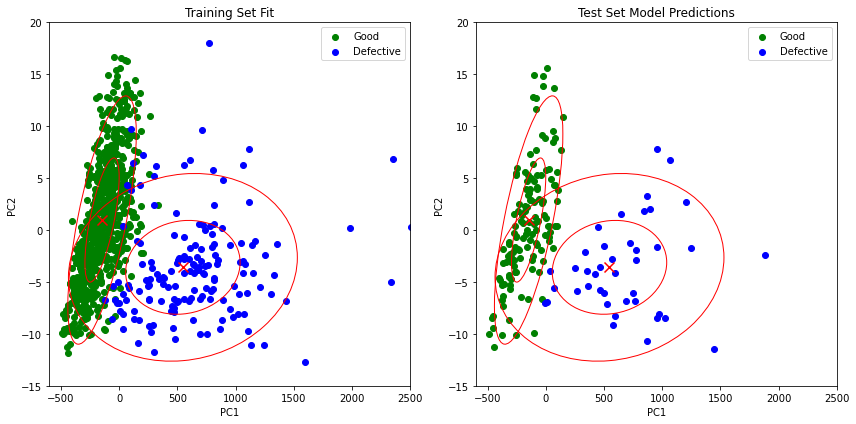
\includegraphics[width=9cm]{classical_img.png}
    \centering
    \caption{The left plot shows the transformed training set with the GMM fit to it. The class names were not given, as it was unsupervised but the true labels were displayed for visualization purposes. The right plot shows the transformed test set and the prediction made by the clustering model.}
\label{fig:recon}
\end{figure}

This framework has established a robust baseline for identifying effective combinations of feature extraction and clustering techniques with classical methods.

\subsection{Autoencoder}
An autoencoder is trained in a self-supervised fashion; the output is expected to be the same as the input. 
We then calculate the error in this reconstruction, and backpropagate this error through the network to update individual weights. 
An example reconstruction is shown in Figure \ref{fig:recon}.

\begin{figure}[h]
    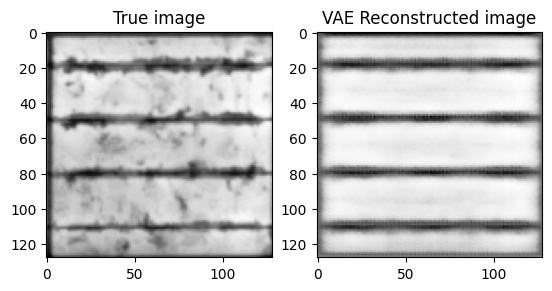
\includegraphics[width=9cm]{recon.png}
    \centering
    \caption{A reconstructed cell that is experiencing significant busbar corrosion}
\label{fig:recon}
\end{figure}
Note that this reconstruction does \textit{not} consider cell type, as the true image is polycrystalline Si and the reconstruction appears to be monocrystalline Si. 
This is a notable finding that also appears in the classical image processing methodology. 
In this use case, the behaviour is to be encouraged as we are trying to cluster failures, not cell type. 
Further note that the edges of the reconstructed image are not sharp; this is a consequence of choosing a Variational Autoencoder, which seeks to minimize expected failures by learning fuzzy borders. 
This flaw could be reduced by integrating an adversarial component at the cost of training instability. 
The training curve for this model is plotted in Figure \ref{fig:loss}. 
Note that early stopping was applied on this model (and so the relative magnitude of the loss is still large) to avoid overfitting on very small datasets. 

\begin{figure}[H]
    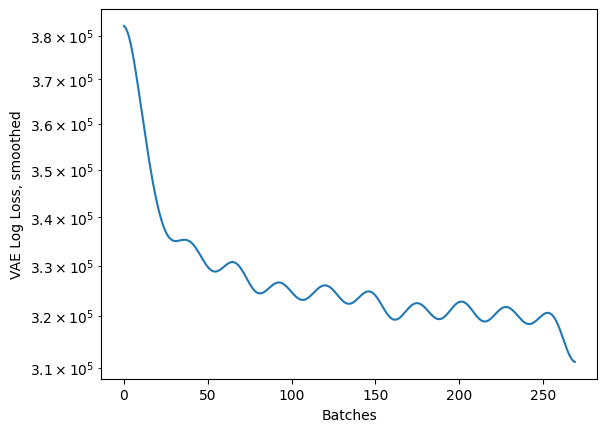
\includegraphics[width=9cm]{loss_curve.png}
    \centering
    \caption{Model loss curve, where the loss term is a sum of a reconstructive binary crossentropy and a KL divergence between the true and learned noise as a part of the variational method. 
    Convergence to large loss values indicate a lack of data in the training set, a typical issue in small-scale datasets like this. Note that an exact reconstruction is not needed for this work, so blurred or idealized representations of the image are acceptable, provided that the encoded feature vector remain useful.}
\label{fig:loss}
\end{figure}

A major hyper-parameter for this type of model is the length of the encoded feature vector. 
Generally, the selection process for this parameter is usually similar to that of methods like principal component analysis, as performance at decreasing parameter values is recording in hope of finding a good value. 
In this case, we want to select a value that preserves most of the relevant information, while the feature vector is small enough to analyze. 
Alternatively, a feature vector of length 2 or 3 can be used for visualization, as in Figure \ref{fig:vae_points}. 
\begin{figure}[h]
    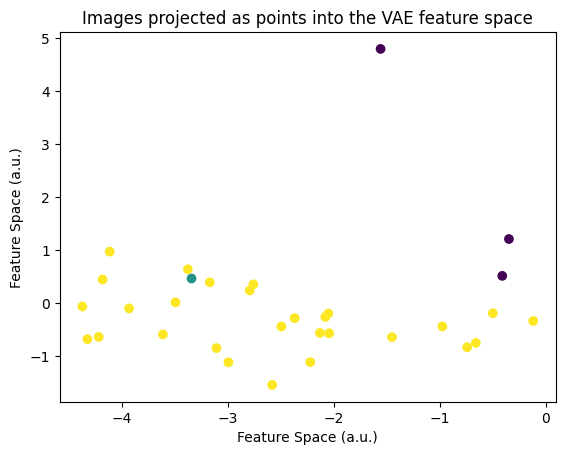
\includegraphics[width=9cm]{cluster_VAE.png}
    \centering
    \caption{Images projected into a learned feature space, where different colors correspond to different failure modes}
\label{fig:vae_points}
\end{figure}
Figure \ref{fig:vae_points} shows good seperation between ``Good" (yellow) and ``Corroded" (purple) cells;  the ``Crack" (teal) cell is mixed in with the "Good" cluster because it shows a very small difference from them. 

\subsection{Clustering}
We choose to evaluate the model in a two-class scenario, representing ``Good" or ``Defective", as shown in Figure \ref{fig:cae_res}.  
This is the most common usage of these models in the field. 
Note that our data has been labeled into three classes for supervised learning, but we are only specifying that the clustering method give two clusters. 
The hope is that the feature embedding are robust and descriptive enough to provide the correct separation between the classes. 
On this task, we find that the \textbf{classical image processing pipeline has an accuracy of 97\%} and the \textbf{CAE/Deep Learning pipeline has an accuracy of 98\%}. 
These values are quite comparable, which shows how both of these models provide robust pipelines for unsupervised ML.

\begin{figure}[h]
    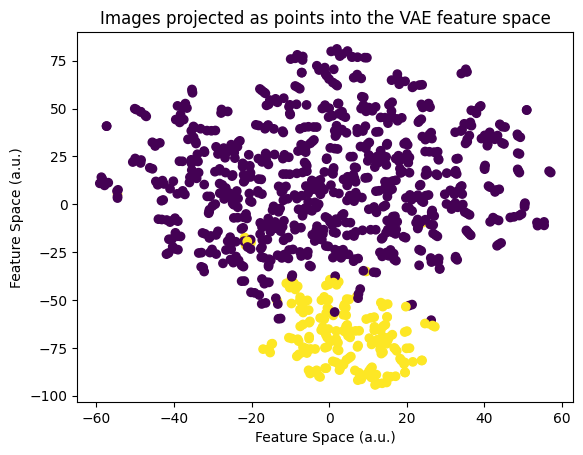
\includegraphics[width=9cm]{whole_dataset.png}
    \centering
    \caption{Clustering result over an entire datset with two clusters}
\label{fig:cae_res}
\end{figure}

\section{Future Work}
In the future, models can be evaluated on larger datasets, which were not included in this study due to copyright concerns\footnote{Companies generally don't like to release datasets where their product is shown to be defective to the public, so much of the data we have is behind an NDA.} or lack of labels. 
The current dataset is quite trivial for these methods, so a more useful comparison may be accomplished with a larger and more difficult dataset. 
Additionally, we would like to better evaluate various clustering methods with various metrics, instead of just classification accuracy.  

Another topic for future work is direct comparison to supervised methods, such as CNNs. 
As noted above, these comparisons are often not one-to-one, as supervised and unsupervised learning are very different paradigms. 
However, simple comparisons like those conducted in this study would be appropriate, and a good topic for full comparative analysis. 


\section{Conclusion}
In this work, we present two pipelines for solar cell electroluminescence (EL) image processing, both of which perform feature extraction, dimensionality reduction, and automated, unsupervised clustering. 
The first pipeline makes use of classical image processing techniques and feature detectors, whereas the second presents a deep learning approach using convolutional/variational autoencoders. 
Model performance is evaluated over an open source dataset, and it is found that both approaches are comparable in accuracy from 97\% to 98\%, which demonstrates the power of unsupervised learning techniques as a class of algorithum. 
Further work includes expansion on more difficult datasets and comparison to supervised convolutional neural network models. 

\section{Group Contributions}
\begin{enumerate}
    \item Benjamin Pierce: Deep Learning/CAE pipeline, project conceptualization, writing, slides
    \item Ellis Wright: Classical Image Processing pipeline, live demo, slides
    \item Rounak Chawla: Paper edits
\end{enumerate}

\section{Acknowledgements}
BGP would like to acknowledge Dr. Jennifer Braid, Dr. Norman Jost, and Emma Cooper at Sandia National Laboratories for continued discussions and code review on electroluminescence image processing via funding from the DuraMAT consortium, as well as Dr. Ahmad Karimi at Oak Ridge National Laboratory for original dataset curation and publication to OSF. 

This work made use of the High Performance Computing Resource in the Core Facility for Advanced Research Computing at Case Western Reserve University

This material is based upon work supported by the National Science Foundation Graduate Research Fellowship under Grant No. 1937968.

\section{Appendix}
Code written and data utilized for this project can be found on our GitHub page: \href{https://github.com/bgpierc/cwru-csds490-project}{https://github.com/bgpierc/cwru-csds490-project}

The primary dataset utilized in this project can be found via the OSF at: \href{https://osf.io/4qrtv/}{https://osf.io/4qrtv/}

\bibliography{refs_490_final} % Entries are in the refs.bib file
\end{document}